\documentclass[tikz,border=8pt]{standalone}
% Shared styles for the Hands-On 4 diagrams. Colours match the Hands-On 1 diagrams.
\usepackage{amsmath,amssymb}
\usetikzlibrary{positioning,calc,arrows.meta,decorations.pathreplacing,shapes.geometric}
\definecolor{tensorblue}{HTML}{3274B5}
\definecolor{envblue}{HTML}{1E4C7C}
\definecolor{opteal}{HTML}{357A76}
\tikzset{
  leg/.style={line width=1.7pt},
  thinedge/.style={line width=1.0pt},
  tensor/.style={circle,draw,line width=1.5pt,fill=tensorblue,minimum size=9mm,inner sep=0},
  vertex/.style={circle,draw,line width=1.0pt,fill=white,minimum size=6mm,inner sep=0,font=\small},
  copy/.style={circle,draw,line width=1.5pt,fill=black,minimum size=3.6mm,inner sep=0},
  op/.style={rectangle,draw,line width=1.5pt,fill=opteal,minimum size=5.6mm,inner sep=0},
  % messages are triangles pointing in the direction the message travels
  msg/.style={isosceles triangle,isosceles triangle apex angle=75,draw,line width=1.5pt,fill=envblue,inner sep=0,
              minimum width=8mm,minimum height=10mm,shape border rotate=0},
  msgl/.style={msg,shape border rotate=180},
  msgu/.style={msg,shape border rotate=90},
  msgd/.style={msg,shape border rotate=270},
  % a matrix message: a slightly larger triangle, its two legs fan out from it
  msgmat/.style={msg,minimum width=10mm,minimum height=13mm},
  lab/.style={font=\large},
  code/.style={font=\ttfamily\large},
  arrow/.style={-{Latex[length=3mm]},line width=1.2pt},
}

\begin{document}
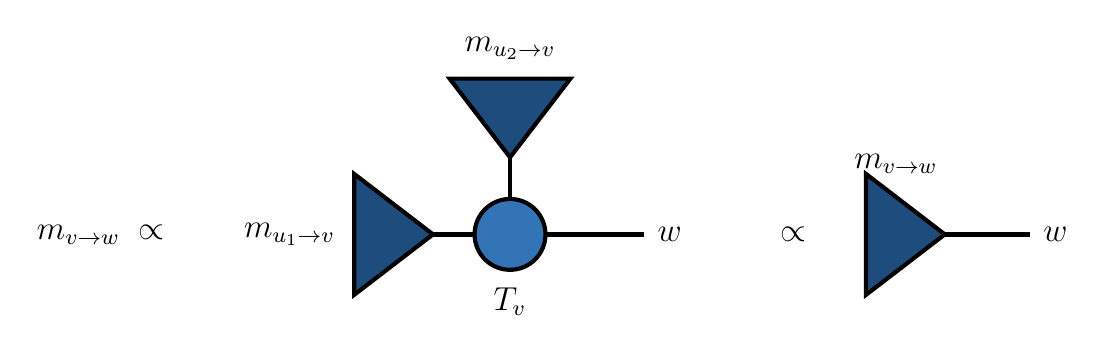
\begin{tikzpicture}
  \node[lab] at (-2.2,0) {$m_{v \to w} \;\propto$};
  % T_v with legs left (from u1), up (from u2), right (to w); legs first, nodes on top
  \coordinate (T) at (3.0,0);
  \draw[leg] (T) -- ++(-1.6,0);
  \draw[leg] (T) -- ++(0,1.6);
  \draw[leg] (T) -- ++(1.7,0);
  \node[tensor] at (T) {};
  \node[lab] at (3.0,-0.85) {$T_v$};
  \node[msg]  at (1.4,0) {};
  \node[msgd] at (3.0,1.6) {};
  \node[lab,anchor=east] at (0.9,0) {$m_{u_1 \to v}$};
  \node[lab,anchor=south] at (3.0,2.1) {$m_{u_2 \to v}$};
  \node[lab,anchor=west] at (4.75,0) {$w$};
  % result: a single message on the leg towards w
  \node[lab] at (6.6,0) {$\propto$};
  \coordinate (M) at (7.9,0);
  \draw[leg] (M) -- ++(1.7,0);
  \node[msg] at (M) {};
  \node[lab,anchor=south] at (7.9,0.65) {$m_{v \to w}$};
  \node[lab,anchor=west] at (9.65,0) {$w$};
\end{tikzpicture}
\end{document}
